\documentclass[]{report}
\usepackage{kotex}
\usepackage{verbatim} 
\usepackage{graphicx} 

\usepackage{listings}
\usepackage{color}

\definecolor{dkgreen}{rgb}{0,0.6,0}
\definecolor{gray}{rgb}{0.5,0.5,0.5}
\definecolor{mauve}{rgb}{0.58,0,0.82}

\lstset{frame=tb,
	language=Python,
	aboveskip=3mm,
	belowskip=3mm,
	showstringspaces=false,
	columns=flexible,
	basicstyle={\small\ttfamily},
	numbers=none,
	numberstyle=\tiny\color{gray},
	keywordstyle=\color{blue},
	commentstyle=\color{dkgreen},
	stringstyle=\color{mauve},
	breaklines=true,
	breakatwhitespace=true,
	tabsize=3
}


% Title Page
\title{HW02 - REPORT}
\author{정보컴퓨터공학부 201624536 이국현}


\begin{document}
\maketitle

\chapter{서론}
\begin{itemize}
	\item 이미지 필터
	\item Low Pass Filter
	\item High Pass Filter
\end{itemize}
\
\section{이미지 필터}

\begin{figure}[ht!]
	\centering
	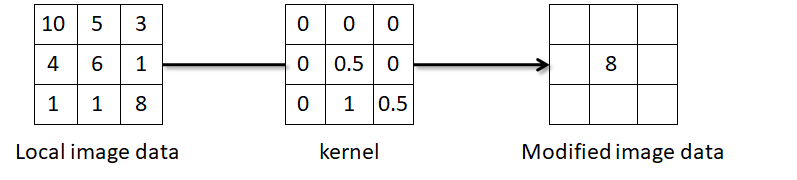
\includegraphics[width=1\textwidth]{image/filtering.png}
	\caption{Filtering}
	\label{filtering}
\end{figure}

이미지의 각 범위에 만들어둔 filter(kenel)를 이용해 cross-correlation 또는 convolution을 수행하여 특별한 처리를 할 수 있다. \\

\section{Low Pass Filter}

\begin{figure}[ht!]
	\centering
	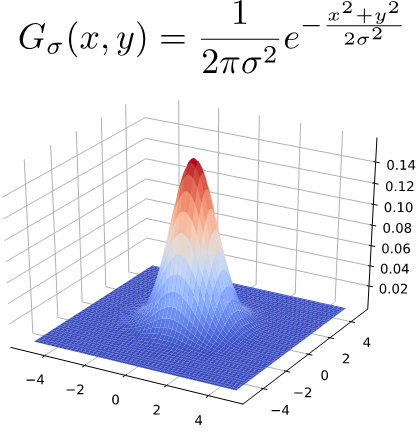
\includegraphics[width=0.5\textwidth]{image/gaussianFilter.png}
	\caption{Gaussian Filter}
	\label{gaussianFilter}
\end{figure} 

Gaussian Filter를 이용하면 각 pixel에 인접한 pixel을 반영하여 변화를 줄임으로써 Low Pass Filter를 구현할 수 있다. \\

\section{High Pass Filter}
\begin{figure}[ht!]
	\centering
	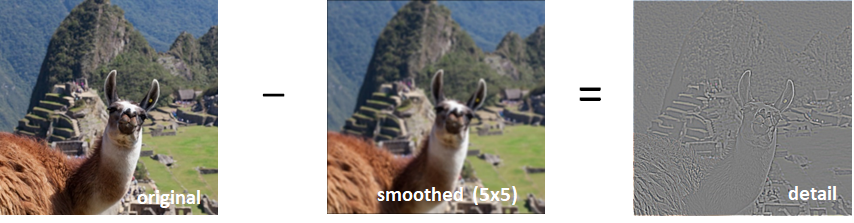
\includegraphics[width=1\textwidth]{image/highPassFilter.png}
	\caption{High Pass Filter}
	\label{highPassFilter}
\end{figure} 

High Pass Filter 역시 filter(kernel)을 구현할 있지만, 가장 기본적인 방법으로 원본 이미지에서 Low Frequency Image를 빼서 High Frequency Image를 구할 수 있다. \\


\chapter{본론}
\section{Part 1: Gaussian Filtering}
\subsection*{1-1) boxfilter(n)}
\begin{lstlisting}
def boxfilter(n):
	assert n % 2 == 1, "Dimension must be odd"
	# element의 합은 1이 되도록 normalize
	value = 1 / n**2
	return np.full((n, n), value)
\end{lstlisting}

\begin{figure}[ht!]
	\centering
	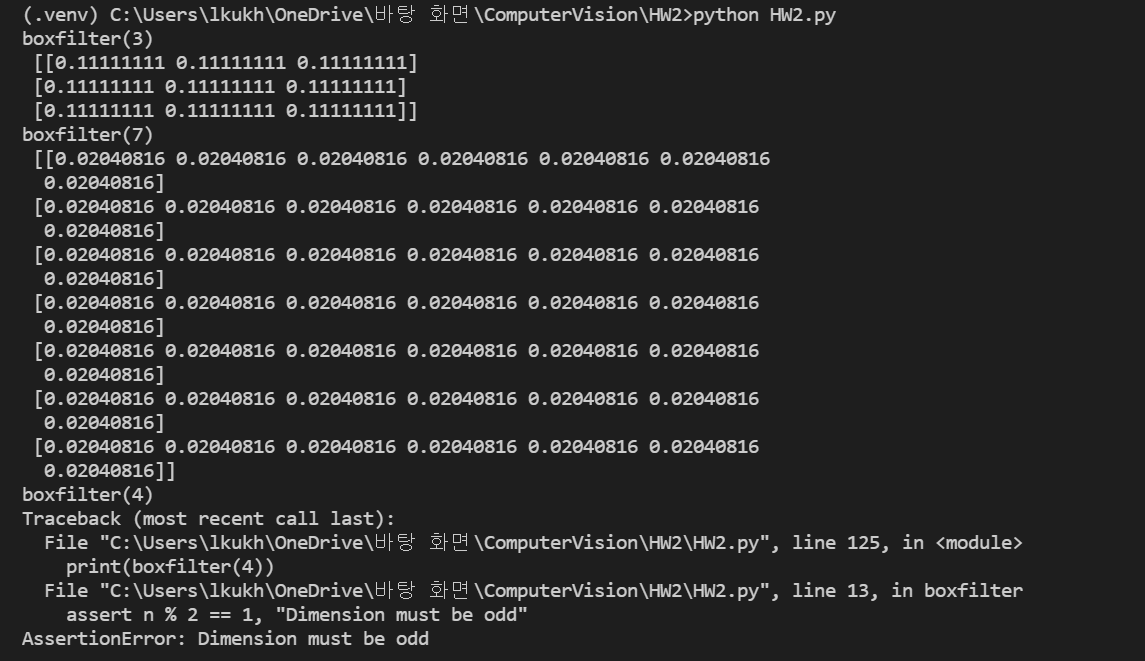
\includegraphics[width=1\textwidth]{image/result_1-1.png}
	\caption{Result 1-1}
	\label{result1_1}
\end{figure}

n x n 크기의 행렬을 만들어주고 n이 짝수일 경우에는 assertion \\

\subsection*{1-2) gauss1d(sigma)}

\begin{lstlisting}
def gauss1d(sigma):
	# sigma * 6을 올림한 값으로 count 설정
	# count가 짝수라면 count에 1을 더해줌
	count = math.ceil(sigma * 6)
	if(count % 2 == 0):
		count += 1
	# 중간값이 0이고 거리가 1멀어질 수록 절대값이 1증가 하도록 배열 생성
	# X^2로 사용하기 때문에 X의 부호는 상관없다
	halfCount = math.floor(count/2)
	X = np.arange(-halfCount, halfCount + 1)
	ndGaussian = np.exp(-X**2/(2*sigma**2))
	# sum으로 나누어 모든 element의 합이 1이 되도록 normalize한다.
	return ndGaussian / ndGaussian.sum()
\end{lstlisting}
sigma 크기에 따라 중간값이 0인 절댓값이 좌우대칭인 배열을 생성하고 다음 식을 적용하였다. 
\[ f(x) = e^{-\frac{X^2}{2\sigma^2}} \] 
앞에 상수를 붙이는 대신 모든 element의 합이 1이 되도록 normalize 해주었다. \\

\begin{figure}[ht!]
	\centering
	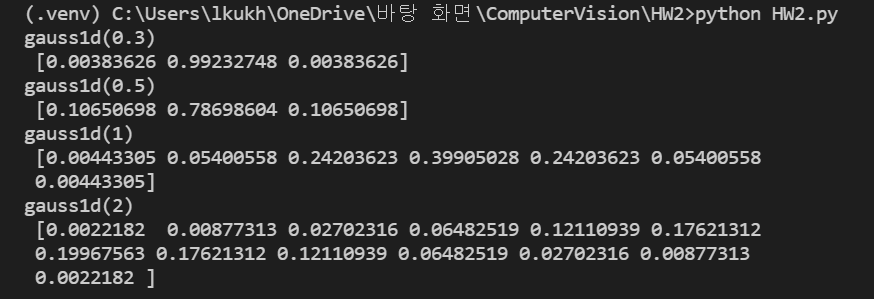
\includegraphics[width=1\textwidth]{image/result_1-2.png}
	\caption{Result 1-2}
	\label{result1_2}
\end{figure}

sigma 값에 따라 배열의 길이가 결정되고, gaussian 식을 normalize 한 값이 저장된다. \\

\subsection*{1-3) gauss2d(sigma)}
\begin{lstlisting}
def gauss2d(sigma):
	# gaussX = e^(-X^2/(2*sigma^2))
	# gaussY = e^(-Y^2/(2*sigma^2))
	# 이므로 외적하면 각 x, y에 대해서 e^(-(X^2 + Y^2)/(2*sigma^2))
	gaussX = gauss1d(sigma)
	gaussY = gauss1d(sigma)
	return np.outer(gaussX, gaussY)
\end{lstlisting}

\[ f(X) = e^{-\frac{X^2}{2\sigma^2}} \] 
\[ f(Y) = e^{-\frac{Y^2}{2\sigma^2}} \] 
두 배열을 외적하여 각 x, y에 대해서 다음 식을 구현하였다.
\[ f(X,Y) = e^{-\frac{X^2 + Y^2}{2\sigma^2}} \] \\

\begin{figure}[ht!]
	\centering
	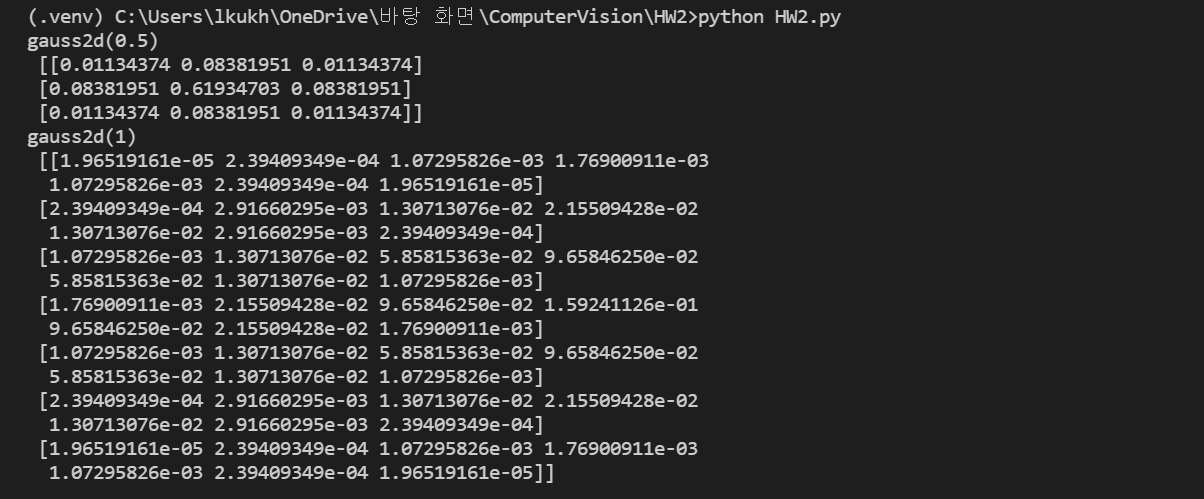
\includegraphics[width=1\textwidth]{image/result_1-3.png}
	\caption{Result 1-3}
	\label{result1_3}
\end{figure}


두 행렬(n)을 외적하여 n x n 행렬을 얻었다. \\



\subsection*{1-4) Blur 처리}
\begin{itemize}
	\item a) convolve2d(array2d, filter)
	\begin{lstlisting}
	def convolve2d(array2d, filter):
		# 연산을 위해 float로 설정
		array2d = array2d.astype(np.float32) 
		filter = filter.astype(np.float32)
		# filter의 크기에 따라 padding 추가
		paddingSize = int((filter[0].size - 1) / 2)
		padded2d = np.pad(array2d, ((paddingSize, paddingSize), (paddingSize, paddingSize)))
		# 원본과 동일한 크기의 result 배열 생성 
		rowSize = array2d.shape[0]
		colSize = array2d.shape[1]
		result2d = np.zeros((rowSize, colSize))
		
		# 모든 픽셀에 주변 영역과 filter를 곱한 배열의 sum으로 값 설정
		# filter가 normalize되어 있기 때문에 mean이 아닌 sum을 사용
		for i in range(0, rowSize):
			for j in range(0, colSize):
				range2d = padded2d[i : i + 2*paddingSize + 1,
		j : j + 2*paddingSize + 1]
		filteredPixel = range2d * filter
		result2d[i][j] = filteredPixel.sum()
		return result2d
	\end{lstlisting}
	
	\begin{figure}[ht!]
		\centering
		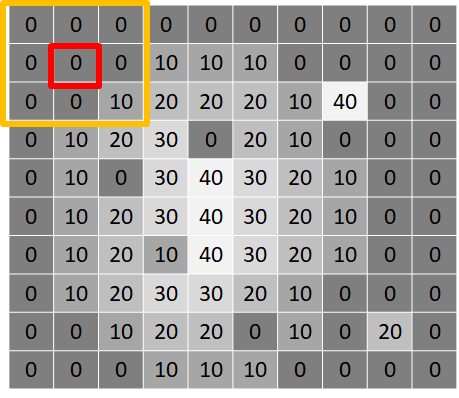
\includegraphics[width=0.5\textwidth]{image/filter.png}
		\caption{filter}
		\label{filter}
	\end{figure}
	convolve2d는 모든 pixel에 대하여 filter를 convolution 한 결과를 반환한다. 먼저 filter와 곱셈 연산을 수행하기 위해 type을 float32로 변환하였다. 그리고 그림 \ref{filter}와 같이 가장자리에 있는 pixel에도 filter를 적용하기 위해 image에 padding을 넣어 convolution을 진행하였다. \\

	\item b) gaussconvolve2d(array2d, sigma)
	
	\begin{lstlisting}
	def gaussconvolve2d(array2d, sigma):
		gaussFilter = gauss2d(sigma)
		return convolve2d(array2d, gaussFilter)
	\end{lstlisting}

	앞에서 만들 함수들을 이용해 sigma 값으로 gaussFilter를 생성하고, 이를 입력받은 이미지에 적용하였다. \\
	
	\item c) 강아지 이미지에 적용한 Blur
	
	\begin{figure}[ht!]
		\centering
		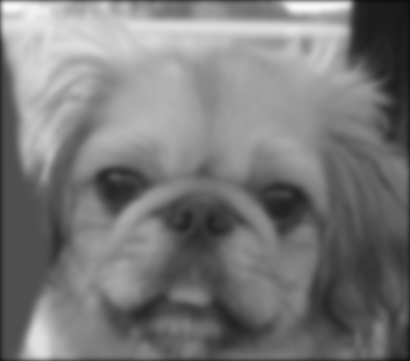
\includegraphics[width=0.5\textwidth]{image/dogGreyBlur.png}
		\caption{Blur sigma=3}
		\label{dogGreyBlur}
	\end{figure}
	강아지 이미지에 sigma 3을 주어 gaussian filter를 적용한 이미지로 blur가 적용된 것을 확인할 수 있다. \\
	
	\item d) 원본 이미지와 Blur 비교
	\begin{figure}[ht!]
		\centering
		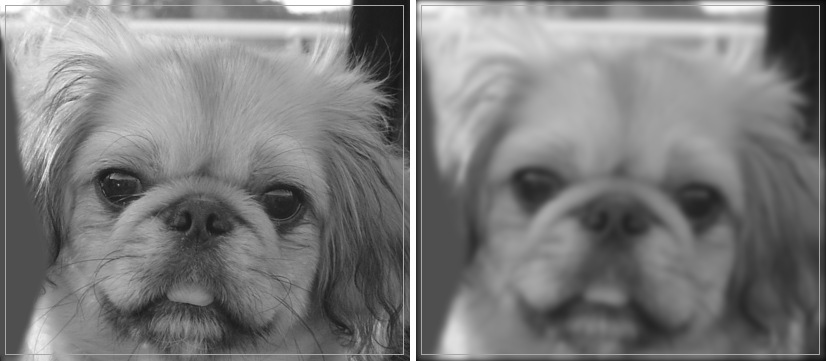
\includegraphics[width=1\textwidth]{image/dogAndBlur.jpg}
		\caption{Origin \& Blur}
		\label{dogAndBlur}
	\end{figure}
	
	원본과 비교했을 때 이미지의 디테일이 사라진 것을 확인할 수 있다. \\
	
\end{itemize}

\section{Part 2: Hybrid Images}

\subsection*{Image Load \& Save}
\begin{lstlisting}
def imgToRGBArray(imagePath):
	# RGB 채널 분리하여 numpy 배열로 변환
	img = Image.open(imagePath)
	imgRGB = img.split()
	arrayRGB = [ np.asarray(channel) for channel in imgRGB ]
	return arrayRGB

def saveImageFromArrayRGB(arrayRGB):
	# overflow, underflow가 일어나지 않도록 값 조정
	for channel in arrayRGB:
		channel[np.where(channel > 255)] = 255
		channel[np.where(channel < 0)] = 0
	# 이미지로 저장하기 위해 type 변환
	arrayRGB = [ channel.astype(np.uint8) for channel in arrayRGB ]
	imgDetail3 = [ Image.fromarray(channel) for channel in arrayRGB ]
	imgDetail = Image.merge("RGB", imgDetail3)
	imgDetail.show()
\end{lstlisting}
이미지에서 RGB를 각각 처리하기 위해 이미지를 불러와 RGB 채널로 분리하여 array로 변환하는 함수를 작성하였다. 그리고 처리가 완료된 array를 합쳐 이미지로 만드는 함수를 작성하였다. 이때 처리가 완료된 array는 값의 범위가 1byte를 벗어날 수 있기 때문에, 이미지로 변환하기 전에 overflow 또는 underflow가 일어날 값에서 최댓값, 최솟값으로 변환해 해주었다. \\

\subsection*{1) Low Pass Filter}

\begin{lstlisting}
def lowPassFilter(imagePath, sigma):
	originRGB = imgToRGBArray(imagePath)
	# gaussian convolution을 통해 low frequency 필터링
	lowRGB = [ gaussconvolve2d(channel, sigma) for channel in originRGB ]
	return lowRGB
\end{lstlisting}
각각의 채널에 대해 gaussian convolution을 적용해 low frequency filter를 구현하였다. \\

\begin{figure}[ht!]
	\centering
	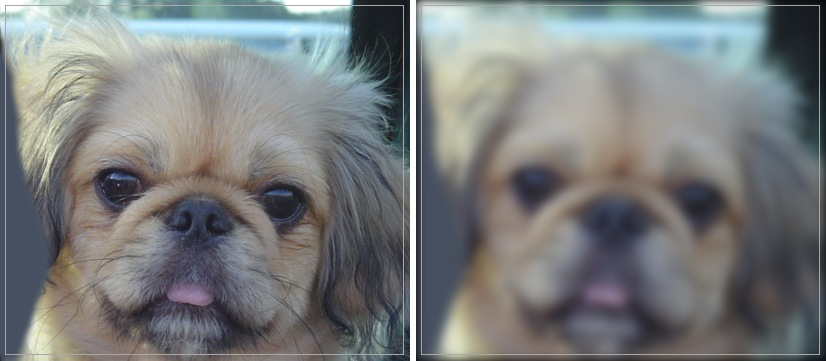
\includegraphics[width=1\textwidth]{image/lowFrequencyDog.jpg}
	\caption{Low Frequency Image}
	\label{lowFrequencyDog}
\end{figure} 

\subsection*{2) High Pass Filter}

\begin{lstlisting}
def highPassFilter(imagePath, sigma):
	originRGB = imgToRGBArray(imagePath)
	# gaussian convolution을 통해 low frequency 필터링
	lowRGB = [ gaussconvolve2d(channel, sigma) for channel in originRGB ]
	# 원본에서 low frequency 이미지를 빼서 high frequence 필터링
	highRGB = [ originRGB[channelNum] - lowRGB[channelNum] for channelNum in range(3) ]
	return highRGB
\end{lstlisting}

각각의 채널에 대해 gaussian convolution을 적용해 low frequency filter를 구하고, 이를 원본 이미지 array에서 빼주어 high frequency image array를 구하였다. \\

\begin{figure}[ht!]
	\centering
	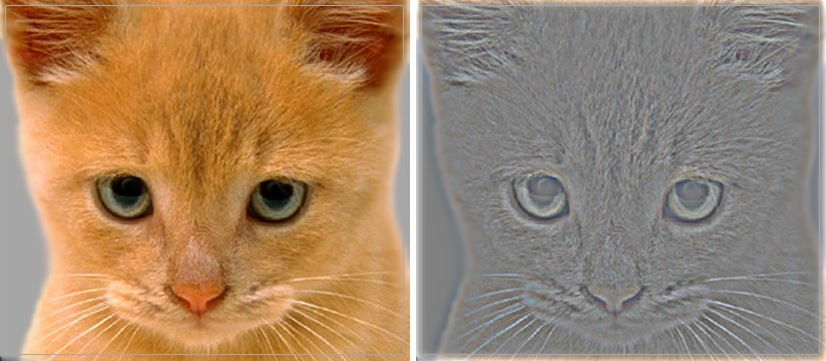
\includegraphics[width=1\textwidth]{image/highFrequencyCat.jpg}
	\caption{High Frequency Image}
	\label{highFrequencyCat}
\end{figure} 

\subsection*{3) Hybrid Image}

\begin{lstlisting}
def makeHybridImage(imagePath1, imagePath2, sigma):
	# low frequency + high frequency
	lowRGB = lowPassFilter(imagePath1, sigma)
	highRGB = highPassFilter(imagePath2, sigma)
	hybridRGB = [ lowRGB[channelNum] + highRGB[channelNum] for channelNum in range(3) ]
	saveImageFromArrayRGB(hybridRGB)
\end{lstlisting}

low frequency image array와 high frequency image array를 더하여 hybrid image를 생성하였다. 이때 각 채널에서의 pixel 값이 범위를 벗어날 수 있기 때문에 saveImageFromArrayRGB에서 범위를 벗어나는 경우 최댓값, 최솟값을 사용하도록 하였다. \\

\begin{figure}[ht!]
	\centering
	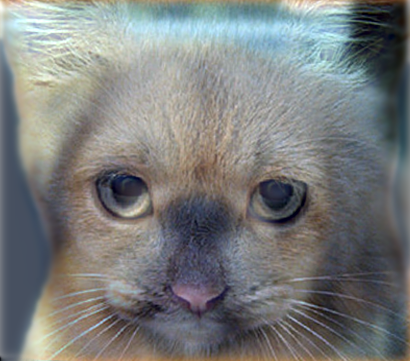
\includegraphics[width=0.6\textwidth]{image/hybridDogCat.png}
	\caption{Hybird Image}
	\label{hybridDogCat}
\end{figure}

큰 사이즈에서는 고양이(high frequency image)로 보이지만 축소하거나 멀리서 보면 강아지(low frequency image)로 보이는 것을 확인할 수 있다.


\chapter{결론}

\section{이미지 처리}

이미지에서 Gaussian Filter를 직접 제작하고고, 이를 이용하여 Low Frequency Filter와 High Frequency Filter를 구현해 보았다. 그리고 Hybrid Image를 제작해 보면서 시각이 인식할 수 있는 Image Frequency에 대해 알 수 있었다. 


\section{주의 사항}
이미지를 처리할 때는 Data Type 사용에 주의할 필요가 있다. 이미지의 각 채널은 1byte를 사용하기 때문에 uint8 type을 사용하지만, 처리 과정에서는 float type으로 변환할 필요가 있다. 그리고 처리가 끝나면 다시 uint8 type으로 변환해야 하는데, 이때 overflow 또는 underflow가 일어나지 않도록 처리할 필요가 있다. \\

\end{document}          
